\let\negmedspace\undefined
\let\negthickspace\undefined
\documentclass[journal]{IEEEtran}
\usepackage[a5paper, margin=10mm, onecolumn]{geometry}
%\usepackage{lmodern} % Ensure lmodern is loaded for pdflatex
\usepackage{tfrupee} % Include tfrupee package

\setlength{\headheight}{1cm} % Set the height of the header box
\setlength{\headsep}{0mm}     % Set the distance between the header box and the top of the text

\usepackage{gvv-book}
\usepackage{gvv}
\usepackage{cite}
\usepackage{amsmath,amssymb,amsfonts,amsthm}
\usepackage{algorithmic}
\usepackage{graphicx}
\usepackage{textcomp}
\usepackage{xcolor}
\usepackage{txfonts}
\usepackage{listings}
\usepackage{enumitem}
\usepackage{mathtools}
\usepackage{gensymb}
\usepackage{comment}
\usepackage[breaklinks=true]{hyperref}
\usepackage{tkz-euclide} 
\usepackage{listings}
% \usepackage{gvv}                                        
\def\inputGnumericTable{}                                 
\usepackage[latin1]{inputenc}                                
\usepackage{color}                                            
\usepackage{array}                                            
\usepackage{longtable}                                       
\usepackage{calc}                                             
\usepackage{multirow}                                         
\usepackage{hhline}                                           
\usepackage{ifthen}                                           
\usepackage{lscape}
\begin{document}

\bibliographystyle{IEEEtran}
\vspace{3cm}

\title{1.11.14}
\author{AI24BTECH11031 - Shivram S
}
% \maketitle
% \newpage
% \bigskip
{\let\newpage\relax\maketitle}

\renewcommand{\thefigure}{\theenumi}
\renewcommand{\thetable}{\theenumi}
\setlength{\intextsep}{10pt} % Space between text and floats


\numberwithin{equation}{enumi}
\numberwithin{figure}{enumi}
\renewcommand{\thetable}{\theenumi}


\textbf{Question: }\\
If the sum of two unit vectors is a unit vector, prove that the magnitude of their difference
is $\sqrt 3$

\textbf{Solution: } \\
Let the two unit vectors be $\vec{a}$ and $\vec{b}$

\begin{align}
    \norm{\vec{a} + \vec{b}}^2 &= 1 \\
    (\vec{a}+\vec{b})^\top(\vec{a}+\vec{b}) &= 1 \\
    \vec{a}^\top\vec{a} + \vec{b}^\top\vec{b} + 2\vec{a}^\top\vec{b} &= 1 \\
    \vec{a}^\top\vec{b} &= \frac{-1}{2}
\end{align}

Hence,

\begin{align}
    \norm{\vec{a} + \vec{b}} &= \sqrt{(\vec{a}-\vec{b})^\top(\vec{a}-\vec{b})} \\
    &= \sqrt{\vec{a}^\top\vec{a} + \vec{b}^\top\vec{b} - 2\vec{a}^\top\vec{b}} \\
    &= \sqrt{1 + 1 - 2 \cdot \frac{-1}{2}} \\
    &= \sqrt{3}
\end{align}

\begin{figure}[h!]
    \centering
    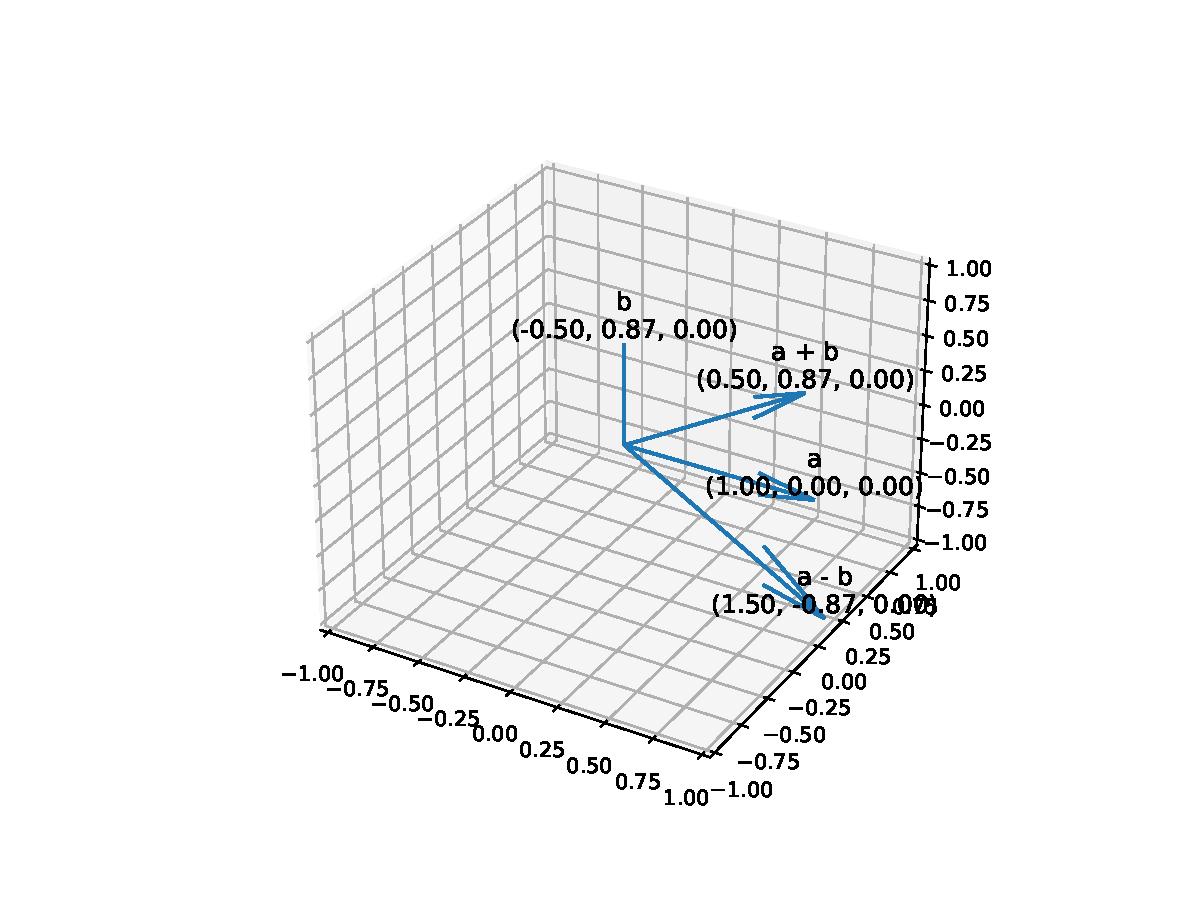
\includegraphics[width=0.7\linewidth]{figs/fig.pdf}
\end{figure}


\end{document}



